\documentclass[aspectratio=169,xcolor=dvipsnames]{beamer}
\usetheme{Madrid}
\usecolortheme{seahorse}
\usepackage{amsmath,amssymb,listings,tikz,pgfplots,booktabs,hyperref}
\usetikzlibrary{arrows.meta,positioning,shapes}
\pgfplotsset{compat=1.18}

\lstset{language=Python,basicstyle=\small\ttfamily,keywordstyle=\color{blue}\bfseries,
  commentstyle=\color{OliveGreen},stringstyle=\color{red},
  frame=single,breaklines=true,showstringspaces=false}

\title[Algorithms -- Week 1]{\textbf{Thiết kế và Phân tích Thuật toán}\\
  \large Week 1: Introduction to Algorithms \& Efficiency Analysis}
\subtitle{TOAE209/TOAH209 -- Foreign Trade University}
\author{Department of Technology \& Data Science}
\date{Semester 2024--2025}
\institute{Foreign Trade University}

\AtBeginSection[]{\begin{frame}<beamer>{Outline}\tableofcontents[currentsection]\end{frame}}

\begin{document}

% ── Title ────────────────────────────────────────────────────────────────────
\begin{frame}\titlepage\end{frame}
\begin{frame}{Outline}\tableofcontents\end{frame}

% ══════════════════════════════════════════════════════════════════════════════
\section{Motivation: Why Algorithms Matter}
% ══════════════════════════════════════════════════════════════════════════════

\begin{frame}{The World Runs on Algorithms}
  \begin{columns}
    \column{0.55\textwidth}
    \begin{block}{Algorithms Are Everywhere}
      \begin{itemize}
        \item Google Search ranks billions of pages in \textbf{< 0.5 seconds}
        \item GPS finds shortest routes across millions of road segments
        \item Netflix recommends content from 200 million+ profiles
        \item Genome sequencing aligns billions of DNA base pairs
        \item Financial trading executes orders in \textbf{microseconds}
      \end{itemize}
    \end{block}
    \column{0.4\textwidth}
    \begin{alertblock}{The Core Question}
      Given a computational problem, how do we solve it \textbf{correctly} and
      \textbf{efficiently}?
    \end{alertblock}
    \vspace{0.5em}
    \begin{exampleblock}{This Course}
      We study \emph{systematic} techniques for designing and analysing
      algorithms that scale to real-world problem sizes.
    \end{exampleblock}
  \end{columns}
\end{frame}

\begin{frame}{A Tale of Two Algorithms}
  \textbf{Problem:} Search for a name in a sorted phone book with $n = 10^6$ entries.

  \vspace{0.8em}
  \begin{columns}
    \column{0.45\textwidth}
    \begin{block}{Linear Search}
      Check each entry one by one.\\[4pt]
      \textbf{Worst case:} $10^6$ comparisons\\
      At $10^9$ ops/sec: \textbf{1 ms}
    \end{block}
    \column{0.45\textwidth}
    \begin{exampleblock}{Binary Search}
      Repeatedly halve the search space.\\[4pt]
      \textbf{Worst case:} $\log_2(10^6) \approx 20$ comparisons\\
      At $10^9$ ops/sec: \textbf{20 ns}
    \end{exampleblock}
  \end{columns}

  \vspace{1em}
  \begin{center}
    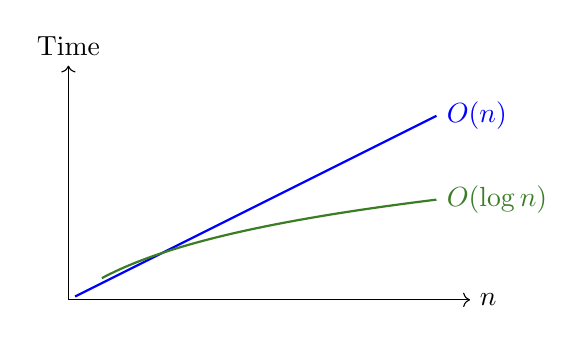
\begin{tikzpicture}[scale=0.85]
      \draw[->] (0,0) -- (6,0) node[right] {$n$};
      \draw[->] (0,0) -- (0,3.5) node[above] {Time};
      \draw[blue,thick,domain=0.1:5.5,samples=100] plot(\x, {\x*0.5}) node[right] {$O(n)$};
      \draw[OliveGreen,thick,domain=0.5:5.5,samples=100] plot(\x,{ln(\x+1)*0.8}) node[right] {$O(\log n)$};
    \end{tikzpicture}
  \end{center}
\end{frame}

% ══════════════════════════════════════════════════════════════════════════════
\section{Historical Development}
% ══════════════════════════════════════════════════════════════════════════════

\begin{frame}{A Brief History of Algorithms}
  \begin{description}[leftmargin=2cm]
    \item[300 BC] Euclid's GCD algorithm -- one of the oldest known
    \item[9th c.\ AD] Al-Khwarizmi (الخوارزمي) names the discipline
    \item[1843] Ada Lovelace writes the first computer program (Bernoulli numbers)
    \item[1936] Alan Turing formalises computation with the Turing machine
    \item[1945] Merge Sort invented by John von Neumann
    \item[1956] Dijkstra's shortest path algorithm
    \item[1971] Cook's theorem -- foundations of NP-completeness
    \item[1973] Knuth's \emph{The Art of Computer Programming} -- TAOCP
    \item[1990] Introduction to Algorithms (CLRS) -- the course textbook
    \item[2010s] Algorithm design for machine learning, quantum computing
  \end{description}
\end{frame}

% ══════════════════════════════════════════════════════════════════════════════
\section{What Is an Algorithm?}
% ══════════════════════════════════════════════════════════════════════════════

\begin{frame}{Definition and Properties}
  \begin{block}{Definition (CLRS)}
    An \textbf{algorithm} is any well-defined computational procedure that takes
    some value (or set of values) as \emph{input} and produces some value (or
    set of values) as \emph{output}.
  \end{block}

  \vspace{0.5em}
  \textbf{Properties an algorithm must satisfy:}
  \begin{enumerate}
    \item \textbf{Correctness} -- produces the correct output for every valid input
    \item \textbf{Definiteness} -- each step is precisely defined
    \item \textbf{Finiteness} -- terminates after a finite number of steps
    \item \textbf{Effectiveness} -- each step can be carried out mechanically
    \item \textbf{Input / Output} -- zero or more inputs, one or more outputs
  \end{enumerate}

  \vspace{0.5em}
  \begin{exampleblock}{Algorithm vs Program}
    An \textit{algorithm} is a mathematical concept; a \textit{program} is its
    implementation in a specific language on a specific machine.
  \end{exampleblock}
\end{frame}

\begin{frame}[fragile]{Example: Insertion Sort}
  \begin{columns}
    \column{0.52\textwidth}
    \begin{lstlisting}
def insertion_sort(A):
    for j in range(1, len(A)):
        key = A[j]
        i = j - 1
        while i >= 0 and A[i] > key:
            A[i+1] = A[i]
            i -= 1
        A[i+1] = key
    return A
    \end{lstlisting}
    \column{0.44\textwidth}
    \textbf{Loop invariant:}\\
    At the start of each iteration, \texttt{A[0..j-1]} contains the original
    elements of \texttt{A[0..j-1]} in \textbf{sorted order}.

    \vspace{0.5em}
    \begin{itemize}
      \item \textbf{Initialisation}: trivially true for $j=1$
      \item \textbf{Maintenance}: inserting \texttt{key} preserves order
      \item \textbf{Termination}: $j=n$, array fully sorted
    \end{itemize}
  \end{columns}
\end{frame}

% ══════════════════════════════════════════════════════════════════════════════
\section{Efficiency: Time \& Space Complexity}
% ══════════════════════════════════════════════════════════════════════════════

\begin{frame}{Why Efficiency Matters -- The Scale Problem}
  \begin{table}
    \centering
    \caption{Running time for different complexities ($10^9$ ops/sec)}
    \begin{tabular}{lrrrr}
      \toprule
      Complexity & $n=10$ & $n=100$ & $n=1\,000$ & $n=10^6$ \\
      \midrule
      $O(\log n)$ & 3 ns & 7 ns & 10 ns & 20 ns \\
      $O(n)$      & 10 ns & 100 ns & 1 $\mu$s & 1 ms \\
      $O(n\log n)$ & 33 ns & 665 ns & 10 $\mu$s & 20 ms \\
      $O(n^2)$    & 100 ns & 10 $\mu$s & 1 ms & \textbf{17 min} \\
      $O(n^3)$    & 1 $\mu$s & 1 ms & 1 sec & \textbf{31 years} \\
      $O(2^n)$    & 1 $\mu$s & $10^{14}$ yrs & $\infty$ & $\infty$ \\
      \bottomrule
    \end{tabular}
  \end{table}

  \begin{alertblock}{Key Insight}
    Algorithm choice dominates hardware speed. A faster computer running a worse
    algorithm often loses to a slower computer running a better one.
  \end{alertblock}
\end{frame}

\begin{frame}{Models of Computation}
  \textbf{RAM Model (Random Access Machine):}
  \begin{itemize}
    \item Each basic operation (arithmetic, comparison, assignment, memory access)
          costs \textbf{one unit of time}
    \item Memory is infinite and uniformly accessible
    \item Allows us to analyse algorithms \emph{independently of hardware}
  \end{itemize}

  \vspace{0.8em}
  \textbf{Two key metrics:}
  \begin{columns}
    \column{0.45\textwidth}
    \begin{block}{Time Complexity $T(n)$}
      Number of basic operations as a function of input size $n$.
    \end{block}
    \column{0.45\textwidth}
    \begin{block}{Space Complexity $S(n)$}
      Amount of extra memory used as a function of $n$ (beyond the input).
    \end{block}
  \end{columns}

  \vspace{0.8em}
  \textbf{Analysis cases:}
  \begin{itemize}
    \item \textbf{Worst case} $T_{\text{worst}}(n)$ -- maximum over all inputs of size $n$
    \item \textbf{Average case} $T_{\text{avg}}(n)$ -- expected over random inputs
    \item \textbf{Best case} $T_{\text{best}}(n)$ -- minimum (rarely used alone)
  \end{itemize}
\end{frame}

\begin{frame}{Counting Operations: Insertion Sort}
  \begin{table}
    \small
    \begin{tabular}{lcc}
      \toprule
      Statement & Cost & Times \\
      \midrule
      \texttt{for j in range(1, n):}            & $c_1$ & $n$ \\
      \quad\texttt{key = A[j]}                   & $c_2$ & $n-1$ \\
      \quad\texttt{i = j - 1}                    & $c_3$ & $n-1$ \\
      \quad\texttt{while i>=0 and A[i]>key:}     & $c_4$ & $\sum_{j=1}^{n-1} t_j$ \\
      \quad\quad\texttt{A[i+1] = A[i]}           & $c_5$ & $\sum_{j=1}^{n-1} (t_j-1)$ \\
      \quad\quad\texttt{i -= 1}                  & $c_6$ & $\sum_{j=1}^{n-1} (t_j-1)$ \\
      \quad\texttt{A[i+1] = key}                 & $c_7$ & $n-1$ \\
      \bottomrule
    \end{tabular}
  \end{table}

  \textbf{Worst case} (reverse-sorted): $t_j = j$, giving $T(n) = an^2 + bn + c = \Theta(n^2)$\\
  \textbf{Best case} (already sorted): $t_j = 1$, giving $T(n) = dn + e = \Theta(n)$
\end{frame}

% ══════════════════════════════════════════════════════════════════════════════
\section{Asymptotic Notation (Preview)}
% ══════════════════════════════════════════════════════════════════════════════

\begin{frame}{Asymptotic Notation -- First Look}
  We care about \textbf{growth rate} as $n \to \infty$, not exact constants.

  \vspace{0.5em}
  \begin{columns}
    \column{0.3\textwidth}
    \begin{block}{$O$ (Big-Oh)}
      Upper bound.\\
      $f(n) = O(g(n))$ means $f$ grows \emph{no faster} than $g$.
    \end{block}
    \column{0.3\textwidth}
    \begin{alertblock}{$\Omega$ (Big-Omega)}
      Lower bound.\\
      $f(n) = \Omega(g(n))$ means $f$ grows \emph{at least as fast} as $g$.
    \end{alertblock}
    \column{0.3\textwidth}
    \begin{exampleblock}{$\Theta$ (Theta)}
      Tight bound.\\
      $f(n) = \Theta(g(n))$ means $f$ and $g$ grow at the \emph{same rate}.
    \end{exampleblock}
  \end{columns}

  \vspace{0.8em}
  \begin{center}
    \textbf{Common hierarchy:}\\[4pt]
    $O(1) \subset O(\log n) \subset O(n) \subset O(n\log n) \subset O(n^2) \subset O(n^3) \subset O(2^n) \subset O(n!)$
  \end{center}
\end{frame}

% ══════════════════════════════════════════════════════════════════════════════
\section{Further Reading \& Recent Developments}
% ══════════════════════════════════════════════════════════════════════════════

\begin{frame}{Further Reading}
  \begin{block}{Core Textbook}
    \begin{itemize}
      \item CLRS \textit{Introduction to Algorithms}, 4th ed.\ (2022) -- Ch. 1--3
    \end{itemize}
  \end{block}
  \begin{block}{Supplementary}
    \begin{itemize}
      \item Jeff Erickson, \textit{Algorithms} (free PDF): \url{https://jeffe.cs.illinois.edu/teaching/algorithms/}
      \item Tim Roughgarden, \textit{Algorithms Illuminated} Vol.\ 1
      \item MIT OpenCourseWare 6.006 lecture notes
    \end{itemize}
  \end{block}
  \begin{exampleblock}{Recent Developments}
    \begin{itemize}
      \item \textbf{2022}: Breakthrough $O(n \log n)$ sorting lower bound confirmation
      \item \textbf{2023}: DeepMind AlphaDev discovers faster sorting algorithms via RL
      \item \textbf{2024}: New matrix multiplication algorithm beats Strassen threshold
      \item Algorithm design for \textbf{quantum} and \textbf{neuromorphic} hardware
    \end{itemize}
  \end{exampleblock}
\end{frame}

\begin{frame}{Advanced Topics Preview}
  \begin{itemize}
    \item \textbf{Cache-oblivious algorithms} -- optimal for memory hierarchies
          without knowing cache parameters
    \item \textbf{Online algorithms} -- decisions without knowledge of the future
    \item \textbf{Streaming algorithms} -- single pass over massive data
    \item \textbf{Parallel algorithms} -- PRAM model, work-span analysis
    \item \textbf{Quantum algorithms} -- Shor's factoring, Grover's search
    \item \textbf{Algorithm engineering} -- closing the gap between theory and practice
  \end{itemize}

  \vspace{1em}
  \begin{alertblock}{Course Roadmap}
    Weeks 1--2: Complexity analysis $\to$ Weeks 3--4: Divide \& Conquer $\to$
    Weeks 5--6: Greedy $\to$ Weeks 7--9: DP $\to$ Weeks 10--11: Graphs $\to$
    Weeks 12--13: Advanced $\to$ Weeks 14--15: Randomised \& Heuristics
  \end{alertblock}
\end{frame}

% ── Summary ──────────────────────────────────────────────────────────────────
\begin{frame}{Week 1 Summary}
  \begin{enumerate}
    \item An \textbf{algorithm} is a finite, well-defined procedure: input $\to$ output
    \item \textbf{Correctness} is proved via loop invariants
    \item \textbf{Time complexity} $T(n)$ counts basic operations in the RAM model
    \item \textbf{Space complexity} $S(n)$ counts extra memory used
    \item \textbf{Asymptotic notation} ($O, \Omega, \Theta$) captures growth rate
    \item Algorithm efficiency can differ by \textbf{orders of magnitude} at scale
  \end{enumerate}

  \vspace{1em}
  \begin{block}{Next Week}
    Formal definitions of $O, \Omega, \Theta$; complexity classes P, NP,
    NP-hard; decidability.
  \end{block}
\end{frame}

\end{document}
